\documentclass[totpages,helvetica,openbib,english]{europecv}
\usepackage[T1]{fontenc}
\usepackage{graphicx}
\usepackage[a4paper,top=1.27cm,left=1cm,right=1cm,bottom=2cm]{geometry}
\usepackage[english]{babel}
\usepackage{bibentry}
\usepackage{url}
\usepackage{enumitem}
\setlist{nolistsep}

\renewcommand{\normalsize}{\fontsize{2.9mm}{3.1mm}\selectfont}

\ecvname{Diego Russo}
\ecvaddress{Via G. Garibaldi 40, 05021, Acquasparta (TR), Italia}
\ecvtelephone[+39 334 5873886]{+39 0744 930614}
\ecvemail{\url{diegor.it@gmail.com} - Personal, gtalk, MSN \\& \url{diego.russo@forinicom.it} - Forinicom S.r.l.}
\ecvhomepage{\url{http://www.diegor.it}}
\ecvnationality{Italian}
\ecvdateofbirth{30 April 1983}
\ecvgender{Male}
\ecvbeforepicture{\raggedleft}
\ecvpicture[width=3cm]{diegor.jpg}
\ecvafterpicture{\ecvspace{-3cm}} 
\ecvfootnote{For more information go to: \url{http://europass.cedefop.eu.int}\\
\textcopyright~European Communities, 2003.}

\begin{document}
    \begin{center}
        \hspace{1pt}
        \vspace{2cm}
    
        {\scshape \textbf{\Huge Diego Russo}}
    
        \vspace{1cm}
    
        {\scshape \textbf{\large \underline{Curriculum Vitae}}}
    
        \vspace{0.25cm}
    
        updated \emph{\textbf{20 March 2010}}
        
        \vspace{2cm}
        
        \begin{figure}[htbp] 
            \begin{center} 
                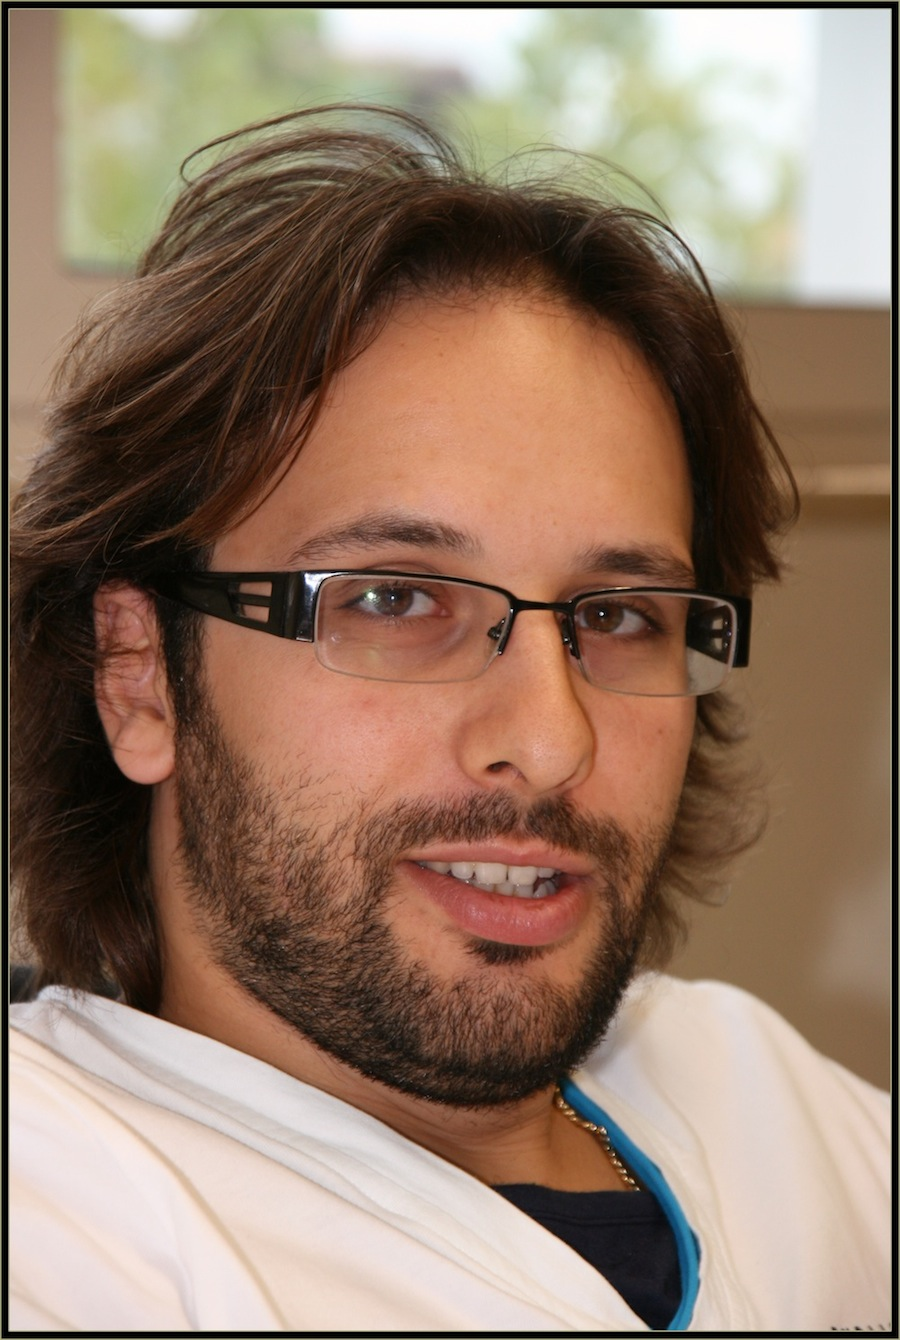
\includegraphics[width=10cm]{io.jpg}
            \end{center} 
        \end{figure}
        
    \end{center}
\pagebreak
\selectlanguage{english}

\begin{europecv}
\ecvpersonalinfo[5pt]

\ecvitem{\large\textbf{Desired employment / Occupational field}}{\large\textbf{Python and Django programmer. Linux and OSX systems engineer. Also open to other employment with opportunities for professional and personal growth.}}

\ecvsection{Work experience}

\ecvitem{Dates}{\textbf{Since 26 April 2008}}
\ecvitem{Occupation or position held}{Programmer, systems engineer (national contract part-time, 25h)}
\ecvitem{Main activities and responsibilities}{Development of a project that aims to provide connectivity and integrated services (video surveillance, VoIP) to public administrations, businesses and individuals. Points provided by the contract
\begin{itemize}
    \item know the products and services in the industry and the business environment: hierarchical and Mesh networks, VoIP services and video surveillance, security of wired and wireless networks;
    \item know and be able to apply the technical fundamentals of professionalism;
    \item know and be able to use techniques and working methods with particular reference to software development and documentation of code;
    \item know and be able to use tools and technologies of work (equipment, machinery and tools), in particular development environment Linux development platform Linux / OSX, programming languages Python and PostgreSQL / MySQL;
    \item know and use measures of individual security and environmental protection;
    \item know about innovations in product, process, context and sector.
\end{itemize}
I also developed applications in python and python-django both the daily work of the technical department and was of pure research and development. In that sense I have implemented from scratch a server to manage the \textbf{hotspot service}}
\ecvitem{Name and address of employer}{Forinicom srl, Via del Popolo, 9 Bastia Umbra, 06083, +390758001868, \url{http://www.forinicom.it}}
\ecvitem[10pt]{Type of business or sector}{Telecommunications}

\ecvitem{Dates}{\textbf{Since 03 September 2009 }}
\ecvitem{Occupation or position held}{Programmer (worker with a project contract, part-time)}
\ecvitem{Main activities and responsibilities}{Development of application management for the municipality of Bettona in django, python, postgresql, linux, apache, for the automatization of management services of master data, building practices, urban planning, calculation of ICI tax and updates cadastral data. Using a version control server (GIT). Also at this stage there was the completion of the product with its marketing.}
\ecvitem{Name and address of employer}{Consorzio Miles - Servizi Integrati, CF 04881101002, Via Rocca di Papa 21, Roma}
\ecvitem[10pt]{Type of business or sector}{Integrated services for public administration}

\ecvitem{Dates}{\textbf{From 11 Dicember 2006 to 31 August 2008}}
\ecvitem{Occupation or position held}{Programmer (worker with a project contract, full-time)}
\ecvitem{Main activities and responsibilities}{Development of application management for the municipality of Bettona in django, python, postgresql, linux, apache, for the automatization of management services of master data, building practices, urban planning, calculation of ICI tax and updates cadastral data. Using a version control server (SVN) with trac and ticket management}
\ecvitem{Name and address of employer}{Consorzio Miles - Servizi Integrati, CF 04881101002, Via Rocca di Papa 21, Roma}
\ecvitem[10pt]{Type of business or sector}{Integrated services for public administration}

\ecvitem{Dates}{\textbf{From 30 July 2006 to 30 Dicember 2006}}
\ecvitem{Occupation or position held}{Undergraduate student (Wireless Broadband Network)}
\ecvitem{Main activities and responsibilities}{Wireless Broadband Network - project \textbf{WeConnect} - Broadband over wifi network:
    \begin{itemize}
        \item Extensive knowledge of the wireless network and its behavior
        \item Good knowledge of laws on the Wi-Fi
        \item Excellent knowledge of the RouterOS system (www.mikrotik.com)
        \item Knowledge of the protocol AAA and the FreeRADIUS server
        \item Administration of various network services: mail (postfix), web server (apache), DNS (pdns), firewall (iptables), database (postgresql), hotspot (chillispot), OS Debian, Voyage (OS for embedded system, Debian based)
    \end{itemize}}
\ecvitem{Name and address of employer}{WEDOIT s.a.s. - Via Protomartiri Francescani,26 - 06088 Assisi (PG)}
\ecvitem[10pt]{Type of business or sector}{Computer science solutions}

\ecvitem{Dates}{\textbf{From 14 November 2005 to 30 May 2006}}
\ecvitem{Occupation or position held}{Trainee (S.E.O. Search Engine Optimization)}
\ecvitem{Main activities and responsibilities}{\vspace{-2mm}
    \begin{itemize}
        \item Basic SEO knowledge. SEO site optimization.
        \item Pagerank and link popularity technics.
        \item System administration of a virtual server, Debian based
        \item Python learning with implementation of some applications SEO oriented.
        \item PHP learning with implementation of some applications SEO oriented
    \end{itemize}}
\ecvitem{Name and address of employer}{WEDOIT s.a.s. - Via Protomartiri Francescani,26 - 06088 Assisi (PG)}
\ecvitem[10pt]{Type of business or sector}{Computer science solutions}

\ecvitem{Dates}{\textbf{March 2002}}
\ecvitem{Occupation or position held}{Trainee (Internship project combined with IFS, Impresa Formativa Simulata - Enterprise Training Simulation)}
\ecvitem{Main activities and responsibilities}{Administration of enterprise network}
\ecvitem{Name and address of employer}{IOSA CARLO S.r.l. - 05100 TERNI - Via Pallotta n. 7 - Tel. (0744) 2460 - Fax (0744) 246035 - P.IVA 00072550551 - \url{http://www.iosacarlo.com} - \url{iosacarlo@iosacarlo.com}}
\ecvitem[10pt]{Type of business or sector}{Waste disposal firm}

\ecvsection{Education and training}

\ecvitem{Dates}{\textbf{Since October 2008}}
\ecvitem{Title of qualification awarded}{Enrolled to specialization of Computer Science, ``Security'' address}
\ecvitem{Principal subjects/occupational skills covered}{Passed following exams with vote:\begin{itemize}
    \item Simulation: 30 cum laude
    \item Advanced programming: 30 cum laude
    \item Advanced Operating Systems: 30 cum laude
    \item Advanced Operating Systems Laboratory: 30 cum laude
\end{itemize}}
\ecvitem{Name and type of organization providing education and training}{University of Perugia, Computer Science department}
\ecvitem[10pt]{Level in national or international classification}{-}

\ecvitem{Dates}{\textbf{Since 17 February 2010}}
\ecvitem{Title of qualification awarded}{Enrolled to 4$^\circ$ module of spanish language}
\ecvitem{Principal subjects/occupational skills covered}{The levels achieved in this form are as follows:
\begin{itemize}
    \item understand the main points of clear standard speech on familiar matters
    \item able to describe experiences and events, reasons and projects
    \item deal with most situations likely to arise whilst traveling in an area where the language is spoken
\end{itemize}}
\ecvitem{Name and type of organization providing education and training}{Comprehensive School ``Volumnio'' Ponte San Giovanni - Perugia}
\ecvitem[10pt]{Level in national or international classification}{-}

\ecvitem{Dates}{\textbf{From August 2009 to March 2010}}
\ecvitem{Title of qualification awarded}{Paper pubblication \textbf{``The AES implementation based on OpenCL for multi/many core architecture''}}
\ecvitem{Principal subjects/occupational skills covered}{Preparing and publication of ``The AES implementation based on OpenCL for multi/many core architecture'' paper for the yearly conference ICCSA 2010 (\url{www.iccsa.org}) at Sangyo University, Fukuoka in Japan. The paper discuss of an implementation of AES algorithm that runs on NVIDIA/ATI graphics card.}
\ecvitem{Name and type of organization providing education and training}{University of Perugia, Computer Science department}
\ecvitem[10pt]{Level in national or international classification}{-}

\ecvitem{Dates}{\textbf{From 14 October 2009 to 12 February 2010}}
\ecvitem{Title of qualification awarded}{Certificate of attendance 42 hours in 50 of the 3$^\circ$ module Spanish language}
\ecvitem{Principal subjects/occupational skills covered}{The reached levels in this module are:
\begin{itemize}
    \item understand sentences and frequently used expressions related to areas of most immediate relevance
    \item can describe in simple terms aspects of their history and own experiences
    \item can speak of the surrounding environment and be able to express needs, intentions and predictions
\end{itemize}}
\ecvitem{Name and type of organization providing education and training}{Comprehensive School ``Volumnio'' Ponte San Giovanni - Perugia}
\ecvitem[10pt]{Level in national or international classification}{-}

\ecvitem{Dates}{\textbf{From August 2007 to August 2008}}
\ecvitem{Title of qualification awarded}{Book publishing \textbf{UbuntuSemplice 7.10} with donation to Canonical Ltd.}
\ecvitem{Principal subjects/occupational skills covered}{\vspace{-2mm}
\begin{itemize}
    \item Contributor, author of many chapters and system engineer of \url{http://www.ubuntusemplice.org/}
    \item Debian virtual server administration
    \item Configuring and using the MediaWiki collaborative software for drawing and composition of the book
    \item Web server Apache configuration
    \item Mailing list configuration to manage the collaborative writing of the book
\end{itemize}}
\ecvitem{Name and type of organization providing education and training}{Ubuntusemplice Project - \url{http://www.ubuntusemplice.org/)}}
\ecvitem[10pt]{Level in national or international classification}{Excellent knowledge of Ubuntu}

\ecvitem{Dates}{\textbf{From February 2007 to July 2007}}
\ecvitem{Title of qualification awarded}{Radio-amateur class A license}
\ecvitem{Principal subjects/occupational skills covered}{Course for radio-amateur
\begin{itemize}
    \item Excellent knowledge of radio technology basics
    \item Excellent knowledge of radio devices and its usage
    \item Basics of phisics and chemical (magnetism,  elettromagnetism)
\end{itemize}}
\ecvitem{Name and type of organization providing education and training}{C.I.S.A.R. Foligno's section}
\ecvitem[10pt]{Level in national or international classification}{SUITABLE, International Callsign \textbf{IZ0OVB}}

\ecvitem{Dates}{\textbf{From 19 March 2007 to 23 March 2007}}
\ecvitem{Title of qualification awarded}{Certificate of attendance to Spanish course}
\ecvitem{Principal subjects/occupational skills covered}{\vspace{-2mm}
\begin{itemize}
    \item Basic grammar of Spanish
    \item The Spanish general culture
\end{itemize}}
\ecvitem{Name and type of organization providing education and training}{Inhispania Intlance S.L / CIF:B83744847 , Montera 10-12, 1-1. 28013, Madrid (Spain)}
\ecvitem[10pt]{Level in national or international classification}{Valutazioni\footnote{Evaluation in accordance with the ``Common European Framework of Reference for Languages''}:
\begin{itemize}
    \item Speaking: A2
    \item Writing: A2
    \item Listening comprehension: A2
    \item Writing comprehension: A2
    \item Oral interaction: A2
\end{itemize}}

\ecvitem{Dates}{\textbf{03-10-25 March 2007}}
\ecvitem{Title of qualification awarded}{Certificate of attendance to Microsoft technology course}
\ecvitem{Principal subjects/occupational skills covered}{Topics covered in the course were:
\begin{itemize}
    \item .NET Framework Architeture (2.0)
    \item ADO.NET
    \item ASP.NET (web forms, Page, controls, security)
    \item C\#
    \item Web Service
    \item Ajax.net
    \item Microsoft Visual Studio 2005
\end{itemize}}
\ecvitem{Name and type of organization providing education and training}{O.S.MO.S.IT, Via Strozzacapponi, 85, 06071 Castel del Piano (Pg)}
\ecvitem[10pt]{Level in national or international classification}{Basics of Microsoft programming}

\ecvitem{Dates}{\textbf{From September 2006 to February 2007}}
\ecvitem{Title of qualification awarded}{\textbf{UbuntuSemplice 6.06} book publishing with donation to Canonical Ltd.}
\ecvitem{Principal subjects/occupational skills covered}{\vspace{-2mm}
\begin{itemize}
    \item Contributor, author of many chapters and system engineer of \url{http://www.ubuntusemplice.org/}
    \item Debian virtual server administration
    \item Configuring and using the MediaWiki collaborative software for drawing and composition of the book
    \item Web server Apache configuration
    \item Mailing list configuration to manage the collaborative writing of the book 
\end{itemize}}
\ecvitem{Name and type of organization providing education and training}{Ubuntusemplice Project - \url{http://www.ubuntusemplice.org/)}}
\ecvitem[10pt]{Level in national or international classification}{Excellent knowledge of Ubuntu}

\ecvitem{Dates}{\textbf{01-02-03 Dicember 2006}}
\ecvitem{Title of qualification awarded}{Certificate of attendance to the course: ISO certifications}
\ecvitem{Principal subjects/occupational skills covered}{Training on security and ISO certifications:
\begin{itemize}
    \item ISO 27001:2005
    \item Policy for Information Security
    \item Risks Analisys (RA)
    \item Analysis of controls of ISO 17799:2005
    \item Risk Transfer Process (RTP)
    \item Certification process
    \item Overview of existing certification audits
    \item Audit plan and checklist
    \item Audit report
    \item A look at the future certifications
\end{itemize}}
\ecvitem{Name and type of organization providing education and training}{WEDOIT s.a.s. - Via Protomartiri Francescani, 26 - 06088 Assisi (PG), Italy}
\ecvitem[10pt]{Level in national or international classification}{Kwoledge of ISO certification process}

\ecvitem{Dates}{\textbf{From October 2002 to November 2006}}
\ecvitem{Title of qualification awarded}{\textbf{Laurea triennale (nuovo ordinamento) in Informatica}}
\ecvitem{Principal subjects/occupational skills covered}{Computer science Bachelor Degree, \textbf{address ``Network''}:
\begin{itemize}
    \item Mathematics (analytical and discrete)
    \item Programming (C, Java, Php, html, xml, xsl, dtd, Pascal, scripting bash and csh, VB.NET, VRML)
    \item Databases (Mysql, MS Access and related programming language)
    \item Networks (ATM, xDSL, Mpls, X.25, Frame Relay), types (wireless, wired) and interaction between them
    \item Knowledge of multimedia system
    \item Overview of parallel computing (mpi)
\end{itemize}}
\ecvitem{Name and type of organization providing education and training}{University of Perugia, Computer Science department}
\ecvitem[10pt]{Level in national or international classification}{\textbf{102/110}}

\ecvitem{Dates}{\textbf{From September 1996 to June 2002}}
\ecvitem{Title of qualification awarded}{\textbf{Accountant graduation programmer (Mercurio project)}}
\ecvitem{Principal subjects/occupational skills covered}{Matters covered by the course (Commercial technical institute) of study as defined by the Ministry of Public Education:
\begin{itemize}
    \item Chemistry / Physics
    \item Mathematics and Laboratory
    \item Biology / Geography astronomical
    \item Word processing and data
    \item Second foreign language (French)
    \item Law and Economics
    \item Business
    \item Economics and Financial Science
    \item Italian Language and Literature
    \item History
    \item Computer Management
    \item Applied Mathematics
    \item First foreign language (English)
    \item Law
\end{itemize}}
\ecvitem{Name and type of organization providing education and training}{Ministry of Public Education - I.T.C. (Commercial technical institute) ``Federico Cesi'', Terni (TR), Italy}
\ecvitem[10pt]{Level in national or international classification}{\textbf{85/100}}

\ecvitem{Dates}{\textbf{From 2001 to 2002}}
\ecvitem{Title of qualification awarded}{Certificate of attendance to the National Project IFS \textbf{Enterprise Training Simulation})}
\ecvitem{Principal subjects/occupational skills covered}{Simulation of waste disposal firm, backed by Iosa Carlo S.r.l. (\url{http://www.iosacarlo.com}).
Within the project I coordinated the work of all students, building the organization chart simulated and programming the website.}
\ecvitem{Name and type of organization providing education and training}{Ministry of Public Education - I.T.C. (Commercial technical institute) ``Federico Cesi'', Terni (TR), Italy}
\ecvitem[10pt]{Level in national or international classification}{-}

\ecvitem{Dates}{\textbf{From 24 September 2001 to 14 October 2001}}
\ecvitem{Title of qualification awarded}{Certificate of attendance to the course as a tutor}
\ecvitem{Principal subjects/occupational skills covered}{Held the activity of tutor/referent of a group of 6 other students/tutors for the building activities of the Italian first class, within the project ``Home, Recovery, Expansion in First Class''.
The activity consisted in assisting teachers of Literature in order to provide valuable support to pupils in lower grades in the use of computers, to perform tasks with the medium-depth multimedia through exercises with a CD-Rom Grammar.}
\ecvitem{Name and type of organization providing education and training}{Ministry of Public Education - I.T.C. (Commercial technical institute) ``Federico Cesi'', Terni (TR), Italy}
\ecvitem[10pt]{Level in national or international classification}{Acquired excellent communication skills, organizational skills and excellent teaching of technical subjects.}

\ecvitem{Dates}{\textbf{From 7 Dicember 2001 to 09 Dicember 2001}}
\ecvitem{Title of qualification awarded}{Certificate of attendance of the ``Pluto Meeting 2001''}
\ecvitem{Principal subjects/occupational skills covered}{Participation in the organization of ``Pluto Meeting 2001''}
\ecvitem{Name and type of organization providing education and training}{Ministry of Public Education - I.T.C. (Commercial technical institute) ``Federico Cesi'', Terni (TR), Italy}
\ecvitem[10pt]{Level in national or international classification}{-}

\ecvitem{Dates}{\textbf{From 26 March 2001 to 02 April 2001}}
\ecvitem{Title of qualification awarded}{Certificate of attendance of the ``Week XI of scientific and technological''}
\ecvitem{Principal subjects/occupational skills covered}{Participation ``Week XI of scientific and technological'', developing both the poster of the week that the provincial program of science in Adobe Photoshop 5.5 and Corel Draw 8.0, engaging in both curricular and extra-curricular hours in the afternoon with great devotion, sense of responsibility, serving also as a reference point for all students of two years who participated in the project.}
\ecvitem{Name and type of organization providing education and training}{Ministry of Public Education - I.T.C. (Commercial technical institute) ``Federico Cesi'', Terni (TR), Italy}
\ecvitem[10pt]{Level in national or international classification}{-}

\ecvitem{Dates}{\textbf{Year 2001}}
\ecvitem{Title of qualification awarded}{Certificate of attendance as a mentor for the computer literacy course for over 65}
\ecvitem{Principal subjects/occupational skills covered}{Computer literacy course in basic counseling work 40 hours total to a group of 30 people aged over 65 years.
I also played the role of Project Coordinator working through the program and coordinating my colleagues.}
\ecvitem{Name and type of organization providing education and training}{Ministry of Public Education - I.T.C. (Commercial technical institute) ``Federico Cesi'', Terni (TR), Italy}
\ecvitem[10pt]{Level in national or international classification}{-}

\ecvitem{Dates}{\textbf{Year 2001}}
\ecvitem{Title of qualification awarded}{Certificate of attendance to the computer course}
\ecvitem{Principal subjects/occupational skills covered}{Computer course in basic counseling work (project 20 students) 30 hours total on office applications (Word, Excel) and Internet}
\ecvitem{Name and type of organization providing education and training}{Ministry of Public Education - I.T.C. (Commercial technical institute) ``Federico Cesi'', Terni (TR), Italy}
\ecvitem[10pt]{Level in national or international classification}{-}

\ecvitem{Dates}{\textbf{16-17-18 November 2000}}
\ecvitem{Title of qualification awarded}{Certificate of attendance to Exposcuola 2000}
\ecvitem{Principal subjects/occupational skills covered}{Exposcuola - Fair comparison of the proposals stem from Europe and the Mediterranean - Arison Paestum hotels}
\ecvitem{Name and type of organization providing education and training}{Ministry of Public Education - I.T.C. (Commercial technical institute) ``Federico Cesi'', Terni (TR), Italy}
\ecvitem[10pt]{Level in national or international classification}{-}

\ecvitem{Dates}{\textbf{From 1997 to 1998}}
\ecvitem{Title of qualification awarded}{Certificate of attendance}
\ecvitem{Principal subjects/occupational skills covered}{Basic Course on multimedia (project 20 students) for a total of 25 hours}
\ecvitem{Name and type of organization providing education and training}{Ministry of Public Education - I.T.C. (Commercial technical institute) ``Federico Cesi'', Terni (TR), Italy}
\ecvitem[10pt]{Level in national or international classification}{-}

\ecvsection{Personal skills and competences}

\ecvmothertongue[5pt]{Italian}
\ecvitem{\large Other language(s)}{\textbf{English, Spanish}}
\ecvlanguageheader{(*)}
\ecvlanguage{English}{\ecvBOne}{\ecvBOne}{\ecvATwo}{\ecvATwo}{\ecvBOne}
\ecvlastlanguage{Spanish}{\ecvBOne}{\ecvBOne}{\ecvATwo}{\ecvATwo}{\ecvBOne}
\ecvlanguagefooter[10pt]{(*)}

\ecvitem[10pt]{Social skills and competences}{Excellent ability to relate to colleagues and associates. Sociable, friendly and good communication skills. Willing to work in teams. My site is a source of continuing social contact and exchange with other technical and less technical.}
\ecvitem[10pt]{Organizational skills and competences}{Ability to work efficiently in different situations.}
\ecvitem[10pt]{Computer skills and competences}{Given my passion for computing in general over the years I have developed a range of skills that vary in many areas of the same.

Since my first computer I had a passion for the open source world and all that concerns him: Indeed I managed machines with \textbf{Linux} distributions such as RedHat 7.3, Slackware 7.1 until you get to Debian machines (from version 3.0 to current ones)

Through this experience I have gained some skill and knowledge in administration \textbf{Linux}: bash scripting, configuring and compiling the kernel, network services, patches for the kernel, C language In addition to regular Linux use \textbf{OSX} for everyday use. Given the continued use and my passion for computers I have in-depth study of OSX-based UNIX systems.

\textbf{I also have a passion for programming}: I know many languages in areas very different from each other as Python, C, PHP, Java, LSL (Linden Scripting Language). The LSL I studied during my activities in \textbf{Second Life}, in fact I worked on several Italian projects in the metaverse as \url{http://www.secundavita.it} Assisi, Milan and Italy Marostica Vera Project.
I have a good knowledge of graphic applications (Gimp, Photoshop) and office tools such as OpenOffice, org and iWork (for OSX)}
\ecvitem[10pt]{Artistic skills and competences}{\vspace{-2mm}
\begin{itemize}
    \item Learning the Spanish language by myself
    \item Amateur photos
    \item Music  (hobby level)
\end{itemize}}

\ecvitem[10pt]{Other skills and competences}{\vspace{-2mm}
\begin{itemize}
    \item Parkour
    \item Music
    \item Willing to learn and study
    \item Attraction for science in general
\end{itemize}}

\ecvitem{Licence(s)}{\vspace{-2mm}
\begin{itemize}
    \item Driving license type B.
    \item Operator license for amateur radio station class A (nr. 020122/AN), International callsign \textbf{IZ0OVB}
\end{itemize}}

\ecvsection{Additional information}

\ecvitem[10pt]{}{\vspace{-10mm}
\begin{itemize}
    \item comply with compulsory military service (referring to studies)
    \item Linux Registered User \#399008
    \item ordinary member of the LUG Perugia
    \item AVIS ordinary member: city council of Acquasparta and member of Avis youth group
    \item marital status: single
\end{itemize}}

\ecvsection{Attachment}
\ecvitem{}{No attachments}

\end{europecv}
\end{document} 